% ============================================================================
% StockFlow --- Technical Report
% INaAI Competition 2026 --- Full-stack Developer Track
% Compile: pdflatex technical_report.tex  (jalankan dari folder backend/docs)
% Hanya menggunakan package standar: geometry, hyperref, enumitem, graphicx,
% booktabs. Tidak ada package esoteric.
% ============================================================================
\documentclass[11pt,a4paper]{article}

\usepackage[margin=2cm]{geometry}
\usepackage{graphicx}
\usepackage{booktabs}
\usepackage{enumitem}
\usepackage[hidelinks]{hyperref}

% Diagram dicari di root project (../../) lebih dulu, lalu folder lokal.
\graphicspath{{../../}{../}{./}}

% Daftar bullet/penomoran lebih rapat agar muat 2-3 halaman.
\setlist{nosep,leftmargin=1.4em,topsep=2pt}

% Header tanpa nomor halaman tebal --- cukup nomor di tengah bawah.
\pagestyle{plain}

\begin{document}

% ---------------------------------------------------------------------------
% Header (bukan cover page)
% ---------------------------------------------------------------------------
\noindent{\Large\textbf{StockFlow --- AI-assisted Inventory Management with Concurrent Safety}}\\[3pt]
\noindent Veri Marpaung \textbar{} INaAI Competition 2026 \textbar{} Full-stack Developer Track \textbar{} 12 Juni 2026

\vspace{4pt}
\hrule
\vspace{8pt}

% ---------------------------------------------------------------------------
% 1. Arsitektur Sistem
% ---------------------------------------------------------------------------
\section*{Arsitektur Sistem}

StockFlow adalah aplikasi web manajemen inventori yang berjalan sebagai \textbf{lima
container Docker} ditambah \textbf{satu layanan LLM eksternal}. Pemisahan service
membuat beban berat (notifikasi, agregasi) terpisah dari jalur permintaan utama.

\begin{itemize}
  \item \textbf{inaai\_frontend} (Next.js App Router, :3000) --- UI di browser, menyimpan token Sanctum dan memanggil API.
  \item \textbf{inaai\_backend} (Laravel + Nginx + PHP-FPM via Supervisord, :8000) --- REST API, validasi, optimistic locking, dan dispatch job.
  \item \textbf{inaai\_worker} (Laravel Queue Worker, image sama dengan backend) --- konsumen job asinkron; hanya membuat notifikasi dan audit, tidak menyentuh jalur transaksi.
  \item \textbf{inaai\_postgres} (PostgreSQL 16, :5432) --- sumber kebenaran data; transaksi ACID untuk operasi stok.
  \item \textbf{inaai\_redis} (Redis 7, :6379) --- berperan ganda: \emph{cache} read-path sekaligus \emph{broker} antrian job.
  \item \textbf{LLM (eksternal)} --- dipanggil oleh backend hanya saat cache insight miss, di luar jalur kritis transaksi.
\end{itemize}

\begin{center}
  % Cek berlapis: (a) compile dari backend/docs/ -> ../../diagram.png,
  % (b) compile dari root project -> diagram.png, (c) tidak ketemu -> fallback teks.
  \IfFileExists{../../diagram.png}{%
    \includegraphics[width=\textwidth]{../../diagram.png}%
  }{\IfFileExists{diagram.png}{%
    \includegraphics[width=\textwidth]{diagram.png}%
  }{%
    \fbox{\parbox{0.95\textwidth}{\ttfamily\footnotesize
      Browser -> Frontend -> Backend\\
      \hspace*{4.5em}Backend -> PostgreSQL  (Query / Transaction)\\
      \hspace*{4.5em}Backend -> LLM (external)  (cache miss / call LLM)\\
      \hspace*{4.5em}Backend -> Redis  (cache \& queue)\\
      \hspace*{4.5em}Redis -> Worker (notification only) -> PostgreSQL  (write notification)
    }}%
  }}
\end{center}

\noindent{\small\textit{Alur:} \emph{request} masuk dari browser ke frontend, diteruskan ke
backend Laravel. Backend menulis/membaca PostgreSQL untuk transaksi, menyimpan hasil read-heavy
ke Redis, dan mendorong \emph{side-effect} ke antrian Redis. Worker mengambil job lalu menulis
notifikasi kembali ke PostgreSQL. LLM hanya disentuh saat menghasilkan insight (cache miss).}

% ---------------------------------------------------------------------------
% 2. Keputusan Teknis Kunci
% ---------------------------------------------------------------------------
\section*{Keputusan Teknis Kunci}

\renewcommand{\arraystretch}{1.25}
\begin{table}[h]
\centering
\small
\begin{tabular}{@{}p{3cm} p{3.8cm} p{8.6cm}@{}}
\toprule
\textbf{Keputusan} & \textbf{Pilihan} & \textbf{Alasan} \\
\midrule
Race condition pada stock-out &
Optimistic locking dengan kolom \texttt{version} &
Konflik \emph{mungkin} terjadi tapi jarang. Satu \texttt{UPDATE} atomik
\texttt{WHERE id=? AND version=? AND stock>=?}; jika \texttt{affected=0} berarti
\emph{stale}, sistem balas 409. Lebih ringan dari pessimistic lock dan tidak
mengunci row di database. \\

Queue \& cache &
Redis dipakai untuk dua peran sekaligus &
Hemat satu service: \emph{broker} antrian job (event-driven) dan \emph{cache}
read-path. Mengurangi kompleksitas operasional tanpa kehilangan kemampuan async. \\

Struktur backend &
Service layer + Repository pattern &
Controller tetap tipis (terima request, panggil, kembalikan). \texttt{StockUpdateService}
memegang logika transaksi; \texttt{ProductRepository} memusatkan query dan cache. Hasilnya
SRP jelas dan mudah dites secara terisolasi. \\

Integrasi AI analytics &
Agregasi data dulu, baru kirim ke LLM &
Backend menyusun ringkasan (daftar low-stock, top-5 transaksi keluar 7 hari, jumlah
transaksi hari ini) sebelum memanggil LLM. Hemat token, lebih deterministik, tidak
membocorkan baris transaksi mentah, dan insight lebih fokus. \\

Isolasi test &
Override \emph{config object}, bukan env var &
\texttt{docker-compose} meng-inject \texttt{DB\_CONNECTION=pgsql} sebagai \emph{system env};
phpdotenv \texttt{ImmutableAdapter} mengalahkan \texttt{force="true"} maupun \texttt{putenv()}.
Solusi: set \texttt{\$app['config']} ke SQLite \texttt{:memory:} \emph{setelah}
\texttt{createApplication()}, ketika config sudah final dan tak dibaca ulang dari env. \\
\bottomrule
\end{tabular}
\end{table}

% ---------------------------------------------------------------------------
% 3. AI Usage Log (ringkasan)
% ---------------------------------------------------------------------------
\section*{AI Usage Log (Ringkasan)}

\textbf{Tool:} Claude (claude.ai, Sonnet 4.6) untuk fase perencanaan; Claude Code
(Sonnet 4.6 \& Opus 4.8) untuk fase coding. \textbf{Pattern:} planning,
architecture-design, generation, debugging, refactoring.

\renewcommand{\arraystretch}{1.2}
\begin{table}[h]
\centering
\small
\begin{tabular}{@{}p{0.9cm} p{1.7cm} p{1.9cm} p{2.4cm} p{8.0cm}@{}}
\toprule
\textbf{Entry} & \textbf{Tool} & \textbf{Pattern} & \textbf{Decision} & \textbf{Dampak} \\
\midrule
1 & Claude Code & generation & ACCEPTED & Inti optimistic locking: \texttt{UPDATE} atomik ber-guard, race ditangani di level DB bukan PHP. \\
2 & Claude Code & debugging & REJECTED $\rightarrow$ MODIFIED & \textbf{Paling impactful} --- perbaiki bug \emph{silent-destructive} test yang menghapus seluruh data PostgreSQL. \\
3 & Claude Code & debugging & MODIFIED & Diagnosis Laravel 11 mengganti \texttt{CACHE\_DRIVER} $\rightarrow$ \texttt{CACHE\_STORE}; diverifikasi ke config, lalu update compose. \\
4 & Claude Code & debugging & ACCEPTED & \texttt{\_\_PHP\_Incomplete\_Class} di worker $\rightarrow$ rebuild image (bukan \texttt{docker cp} per-container). \\
5 & Claude Code & generation & MODIFIED & Ubah service agar mengagregasi data dulu sebelum ke LLM; tambah \texttt{timeout(30)} \& log error. \\
6 & Claude Code & generation & MODIFIED & Output gagal \texttt{tsc} strict (implicit \texttt{any}); diganti destructuring bertipe eksplisit. \\
7 & Claude Code & refactoring & ACCEPTED & Seeder idempotent (\texttt{firstOrCreate}) agar demo clean-state berulang aman. \\
\bottomrule
\end{tabular}
\end{table}

\noindent\textbf{Filosofi.} AI dipakai sebagai \emph{assistant}, bukan pengganti pemahaman ---
setiap baris kode bisa dijelaskan saat Live Defense. Output diterima langsung hanya bila
secara teknis benar dan dapat saya pertanggungjawabkan (Entry 1, 7); dimodifikasi bila
fungsional tapi tidak optimal/aman (Entry 3, 5, 6); dan ditolak bila tidak menyentuh akar
masalah. Empat entri fase perencanaan (P1--P4) juga dicatat di log lengkap, termasuk saat AI
menilai jujur bahwa konteks rancangan saya lebih baik dari versinya. \textbf{Interaksi paling
impactful adalah Entry 2}: saran pertama AI (\texttt{putenv}) saya \emph{tolak} karena setelah
diuji PostgreSQL tetap ter-\emph{wipe}; akar masalahnya adalah urutan bootstrap Laravel dan
\texttt{ImmutableAdapter} phpdotenv. Solusi final (override config object setelah
\texttt{createApplication()}) membuat 44 test \emph{pass} dengan data produksi utuh.

% ---------------------------------------------------------------------------
% 4. Limitasi yang Disadari
% ---------------------------------------------------------------------------
\section*{Limitasi yang Disadari}

\begin{itemize}
  \item \textbf{Cold start free tier} --- deployment gratis dapat menambah latency tidak stabil pada request pertama; klaim p95 stabil tidak berlaku untuk cold start.
  \item \textbf{Respons LLM non-deterministik} --- insight bisa berbeda tiap \emph{regenerate}; tidak cocok dijadikan satu-satunya sumber keputusan operasional.
  \item \textbf{Token di \texttt{localStorage}} --- praktis untuk demo tetapi rentan XSS; idealnya pindah ke cookie \texttt{HttpOnly}.
  \item \textbf{Tidak ada refresh token} --- token tidak ber-rotasi otomatis; sesi panjang harus login ulang secara manual.
  \item \textbf{AI insight bisa stale} --- di-cache 1 jam; bila inventori berubah cepat dalam rentang itu, insight belum mencerminkan kondisi terbaru hingga \emph{regenerate}.
  \item \textbf{Test coverage belum 100\%} --- fokus pada jalur kritis (auth, CRUD, stock, konflik versi, notifikasi); sebagian edge case belum tercakup.
  \item \textbf{Tanpa pagination \& DIP belum penuh} --- \texttt{getAll()} memuat seluruh produk dan repository di-inject sebagai concrete class (bukan interface); cukup untuk skala demo, disadari sebagai langkah lanjutan.
\end{itemize}

% ---------------------------------------------------------------------------
% 5. Skenario Wajib --- Skenario 1 (Zero-Latency Tanpa Async)
% ---------------------------------------------------------------------------
\section*{Skenario Wajib --- Skenario 1 (Zero-Latency Tanpa Async)}

Permintaan ``100\% real-time, tanpa latency sama sekali, dan dilarang memakai websocket,
queue, atau worker'' bersifat \emph{kontradiktif}. Zero-latency mustahil dijanjikan untuk web
production karena setiap request dibatasi fisika jaringan: kecepatan cahaya di fiber,
\emph{round-trip} TCP, dan waktu pemrosesan server. Lebih jauh, \textbf{melarang async justru
memperburuk latency} untuk operasi non-trivial: tanpa queue/worker, semua \emph{side-effect}
(cek threshold, buat notifikasi, audit, agregasi insight) harus dijalankan sinkron di dalam
\emph{request-response cycle}, sehingga request menjadi lambat, mudah \emph{blocking}, dan server
gampang \emph{overload} saat concurrency tinggi. StockFlow menunjukkan kebalikannya: mutasi kritis
(satu \texttt{UPDATE} atomik) tetap sinkron dan kecil sehingga response cepat, sementara kerja berat
dilempar ke Redis queue + worker dan AI insight di-cache di luar jalur kritis. Yang saya
\emph{negosiasikan} bukan menerima constraint secara literal, melainkan menggantinya: zero-latency
menjadi \emph{bounded/predictable latency} yang terukur per jenis operasi (warm runtime, cache hit,
request LLM), dan larangan async menjadi \emph{pemisahan read-path dari write-side-effect}.

\end{document}
